\vspace{1.5cm}

En la figura~\figref{fig:fig_p21}, se muestra el circuito de la fuente de alimentación basado en el \textit{LM723} que armamos usando el mismo driver de corriente que la fuente original y ajustando los resistores de tal forma de que las características de tensión, limitación de corriente, etc, se parezcan lo mas posible al circuito original, los valores de compensación se toman de circuitos recomendados.\\
Con ese circuito, adecuadamente modificado, se repitieron las simulaciones para realizar la comparación pedida.\\

\vfill


\clearpage

\begin{figure}[H] %htb
\begin{center}
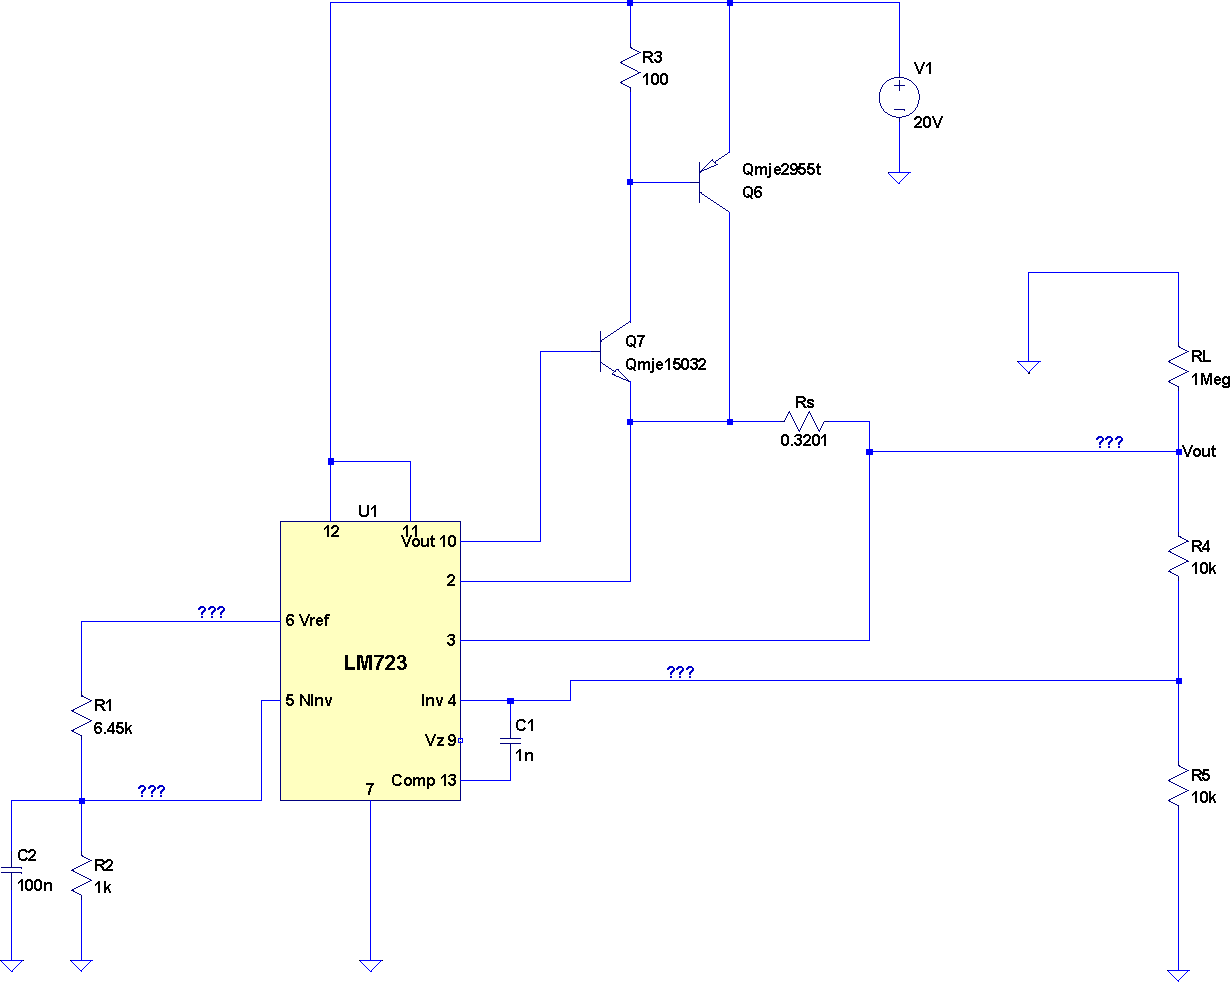
\includegraphics[width=1.2 \textwidth, angle=90]{./img/preguntas/p21.png}
\caption{\label{fig:fig_p21}\footnotesize{Rizado de entrada y salida.}}
\end{center}
\end{figure}

\clearpage

\subsubsection{Punto 6}


En la figura~\figref{fig:fig_p21_p6_output_voltage} se muestra el gráfico de la tensión de salida en modo de regulación de tensión en función de la resistencia del resistor $R_{9}$, el gráfico se obtuvo realizando una simulación paramétrica con $R_{L} = 1 \si[per-mode=symbol]{\mega\ohm}$, con el comando \textbf{SPICE} \textit{.step}, y luego se exportó el resultado y se graficó en \textbf{MATLAB}. En el gráfico se puede apreciar que, como se espera según lo calculado, el crecimiento es lineal con $R_{9}$, entre valores muy cercanos a los nominales de $1 \si[per-mode=symbol]{\volt}$ y $10 \si[per-mode=symbol]{\volt}$.




\vfill

\clearpage

\begin{figure}[H] %htb
\begin{center}
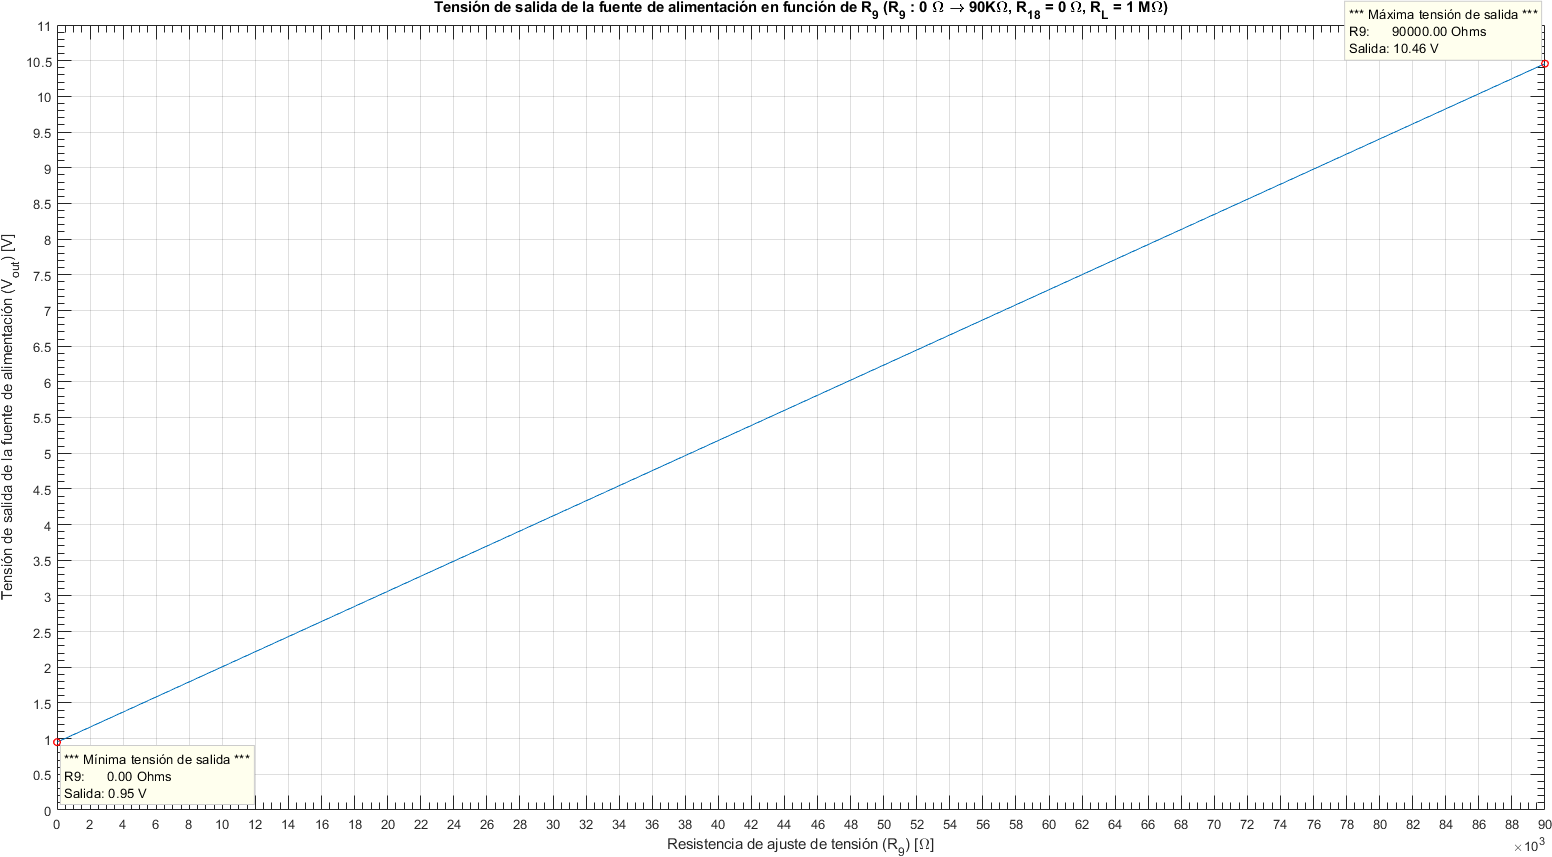
\includegraphics[width=1.2 \textwidth, angle=90]{./img/preguntas/p21_6.png}
\caption{\label{fig:fig_p21_p6_output_voltage}\footnotesize{Tensión de salida, $V_{o}$, en función de $R_{9}$, con esta variando entre $0 \si[per-mode=symbol]{\ohm}$ y $90 \si[per-mode=symbol]{\kilo\ohm}$.}}
\end{center}
\end{figure}



\clearpage